\documentclass[11pt, oneside]{book}   	% use "amsart" instead of "article" for AMSLaTeX format
\usepackage{geometry}                		% See geometry.pdf to learn the layout options. There are lots.
\geometry{letterpaper}                   		% ... or a4paper or a5paper or ... 
%\geometry{landscape}                		% Activate for for rotated page geometry
%\usepackage[parfill]{parskip}    		% Activate to begin paragraphs with an empty line rather than an indent
\usepackage{graphicx}				% Use pdf, png, jpg, or eps§ with pdflatex; use eps in DVI mode
\graphicspath{ {images/} }							% TeX will automatically convert eps --> pdf in pdflatex		
\usepackage{amssymb}

\setlength{\parindent}{0em}

\title{EECS 769 Homework 1}
\author{Elise McEllhiney}
\date{Sept. 8, 2016}							% Activate to display a given date or no date

\begin{document}
\maketitle
\section{Entropy of functions of a random variable}
\textbf{Let $X$ be a discrete random variable.  Show that the entropy of a function of $X$ is less than or equal to the entropy of $X$ by justifying the following steps:
$$H(X,g(X)) = H(X)+H(g(X)|X) = H(X)$$
$$H(X,g(X)) = H(g(X))+H(X|g(X))\geq H(g(X))$$
Thus $H(g(X)) \leq H(X)$.} \\

(a) This is true given the chain rule:  $H(X,Y)=H(X)+H(Y|X)$ proven on page 17 of our textbook.

(b) This is true since $H(g(X)|X)=0$.  $H(g(X)|X)$ is the measure of uncertainty in $g(X)$ given $X$.  Thus, since g(X) is a function of $X$ there is no uncertainty in $g(X)$ if we know $X$.

(c) Also proven given the chain rule $H(X,Y) = H(X)+H(Y|X) = H(Y)+H(X|Y)$.  Joint entropy is not dependent on the order of variables.  Rearranged this is the same as the remark on page 18 that states: $H(X)-H(X|Y)=H(Y)-H(Y|X)$ or that the measure of information provided about $X$ given $Y$ is equal to the amount of information about $Y$ given $X$.

(d) This is true since $H(X|g(X)) \geq 0$.  Entropy is always nonnegative.

\section{Functions}
\textbf{(a) Let $Y=X^7$, where X is a random variable taking on positive and negative integer values.  What is the relationship of $H(X)$ and $H(Y)$?}

\textbf{(b)What if $Y=cos( \pi X/3)$?}

\textbf{(c)What if $Y=cosX$?}

\textbf{(d)What if $Y=X^2$}\\

Since $Y=g(X)$ for all of the given examples, it will always be true that $H(X) \geq H(Y)$ because $H(X) \geq H(g(X))$ as proven above in problem 1.  For (a), since $Y=X^7$ is the same as $X= \sqrt [7] Y$, we know that $H(X)=H(Y)$ since this means that $X=g(Y)$.  That makes X and Y a one-to-one function if $Y=X^7$.  However, (b), (c), and (d) all lose information within the g(X) function and thus $X$ can NOT be described as $g(Y)$.  Therefore, they are not one-to-functions.  The function cos() has a range of return values in a cyclic pattern and thus there is more than one Y for a given X.  Also, (d), being an even power, loses the information about the negativeness of X.  Again this means that there is more than one Y for a given X and that $H(X)>H(Y)$

\section{Mutual information of heads and tails}
\subsection{Consider a fair coin flip.  What is the mutual information between the top side and the bottom side of the coin?}If we know the top side of a fair coin, we will always know what the bottom side of a fair coin is.  If the top side of a fair coin is heads, we can say with certainty that the bottom side is tails.  If the top side is tails, we know that the bottom side is heads.
\subsection{A 6-sided fair die is rolled.  What is the mutual information between the top side and the bottom side?}
Again, if we know the top side of the die, we know the bottom side of the die.  This is assuming that we know the arrangement of the die.  On a typical die we could assume that the top and bottom numbers add to 7, and could therefore give the bottom number on the die with complete certainty given only the top side of the die.
\subsection{What is the mutual information between the top side and the front face (the side that is most facing you)?}

If we know the top side of the die, we know the bottom side of the die with certainty.  However, we do not know which side is facing us.  The mutual information between the top side and the front face is only that the front face cannot be either the number on the top side of the die, nor the number on the bottom side of the die.  For example, if we rolled a 1 on the top side of the die, we know that 6 is on the bottom, and the front face could be 2, 3, 4, or 5.  Assuming a completely fair die and a completely fair roll, these numbers would each have an equal probability (a one in four chance) of being the actual answer.  

\section{Coin Weighing}
\textbf{Suppose one has $n$ coins, among which there may or may not be one counterfeit coin.  If there is a counterfeit coin, it may be either heavier or lighter than the other coins.  The coins are to be weighed by a balance}
\subsection{Count the number of states the $n$ coins can be in, and count the number of outcomes of $k$ weighings.  By comparing them, find an upper bound on the number of coins $n$ so that $k$ weighings will find the counterfeit coin (if any) and correctly declare it to be the heavier or lighter}
$n$ coins can be in $2n+1$ states (2n possible options for a counterfeit coin, the 2 is since the coin can be either heavier or lighter; $+1$ for if there is not a counterfeit coin.)  We get 3 possible outcomes per weighing: balance, right side light, right side heavy.  So we get $3^k$ outcomes per k weighings.  From this we can determine that the upper bound of coins $n$ so that $k$ weighings will find the counterfeit coin (if any) and declare it to be heavier or lighter will be: $2n+1 \leq 3^k$
\subsection{(\textit{Difficult and optional}) What is the coin weighing strategy for $k=3$ weighings and 12 coins?}
I am going to number the coins from 1 to 12 for ease of explanation.  Also, in order for this to work, I assume a counterfeit, since proving no counterfeit takes one extra weighing and I couldn't find a way around that, but I figured I'd give it a try anyway.\newline\newline
First, you split the coins into three groups of 4.  Weigh 1,2,3,4 against 5,6,7,8.\newline 
----If they balance, the counterfeit coin is in the group 9,10,11,12.  Weigh 9,10 against 1,2.\newline
--------If they don't balance, the counterfeit is either 9 or 10. Weigh 9 against 1 (known good coin).\newline
------------If they balance, the counterfeit is 10.\newline
------------If they don't balance, the counterfeit is 9\newline
--------If they balance, the counterfeit is either 11,12.  Weigh 11 against 1 (known good coin).\newline
------------If they balance, the counterfeit is 12.\newline
------------If they don't balance, the counterfeit is 11.\newline\newline
----If they don't balance, the counterfeit is 1,2,3,4,5,6,7,8.  Keeping track of which is heavier.  I'll assume 5,6,7,8 to be heavier.  Split the heavier group into two and then two from the lighter group.  Weigh 1,5,6 against 2,7,8.\newline
--------If they balance, either 3 or 4 is counterfeit.  Weigh 3 against 1.\newline
------------If they balance, the counterfeit is 3.\newline
------------If they don't balance, the counterfeit is 4.\newline
--------If they don't balance,  If 2,7,8 is heavier we know either 7 or 8 is heavier, or 1 is lighter and therefore counterfeit.  If 1,5,6 is heavier, we can follow the same logic using the different coins (I don't write out all the possible outcomes since that would be really long).  Weigh 7 against 8.\newline
------------If they balance, 1 is counterfeit.\newline
------------If they don't balance, the heavier coin is counterfeit.\newline\newline
There is one case that we need a fourth weighing to determine if there is no counterfeit coin.  If all three weighings balance, if there is a counterfeit, it must be 12, but we don't know if 12 is counterfeit or not since we have never weighed it.  If the weighings are ever not balanced, we know there is a counterfeit and can forgo the fourth weighing.

\section{Entropy of time to first success}
\textbf{A fair coin is flipped until the first head occurs.  Let $X$ denote the number of flips required}
\subsection{Find the entropy $H(X)$ in bits.  The following expressions may be useful.  $$\sum_{n=1}^{\infty}r^n = r/(1-r), \sum_{n=1}^{\infty}nr^n=r/(1-r)^2$$}

$$p(X=1)=p(heads)=1/2$$
$$p(X=2)=p(tails)*p(heads)=(1/2) * (1/2) = (1/2)^2$$
$$...$$
$$p(X=n)=p(tails)*...*p(heads)=(1/2)^n$$

$$p_X(x)=(1/2)^x$$
$$H(X) = -\sum_{x\epsilon X}p_X(x)log_2p_X(x)= -\sum_{x=1}^{\infty}(1/2)^xlog_2(1/2)^x$$
$$= -\sum_{x=1}^{\infty}(1/2)^xxlog_2(1/2)= -log_2(1/2)\sum_{x=1}^{\infty}(1/2)^xx$$
$$=\sum_{x=1}^{\infty}(1/2)^xx=(1/2)/(1-1/2)^2=2 bits$$
\subsection{Find an "efficient" sequence of yes-no questions of the form, "Is $X$ contained in the set $S$?"  Compare $H(X)$ to the expected number of questions required to determine $X$.}
Since X=1 is the most likely result with probability 0.5, the first question should be "Is $X=1$?".  If incorrect, the next question should be "Is $X=2$?", and so on until the answer is "yes".  The expected number of questions required is equal to $H(X)$.
$$E_Y=\sum_{y=1}^{\infty}y(1/2)^y=(1/2)/(1-1/2)^2 = 2$$
\subsection{Let $Y$ denote the number of flips until the second head appears.  Argue that $H(Y)=H(X_1+X_2) < H(X_1,X_2)=2H(X)$, and interpret in words}
$H(Y)=H(X_1+X_2)$ since flipping coins until you get two heads is the same as flipping for one heads twice, we can conclude that $H(X_1+X_2)$ should be the same as $H(Y)$ or flipping until we get two heads outcomes.  However $H(X_1,X_2)$ as a joint distribution assumes flipping two coins that both land on heads.  This is the same as $2H(X)$ since you are flipping two coins until they both land on heads simultaneously.  Since flipping heads has a probability of 0.5, then flipping two simultaneous heads will have a probability of 0.25.  However, flipping heads. then tails, then heads is still a viable win condition for $Y$ and thus more of the possible outcomes are favorable than two coins at the same time.  Therefore, $H(Y)=H(X_1+X_2) < H(X_1,X_2)=2H(X)$.

\section{Playoff}
\textbf{A playoff consists of a three-game series that terminates as soon as either team wins two games.  Let $X$ be the random variable that represents the outcome of a playoff between teams A and B; examples of possible values of X are AA, and BAB.  Let Y be the number of games played, which ranges from 2 to 3}
\subsection{Assuming that A and B are equally matched and that the games are independent, calculate $H(X),H(Y),H(Y|X)$, and $H(X|Y)$}
\begin{tabular}{| l | c | r }
X & p(X) \\
\hline
AA & 0.25 \\
ABA & 0.125 \\
ABB & 0.125 \\
BAA & 0.125 \\
BAB & 0.125 \\
BB & 0.25 \\
\hline
\end{tabular}
$$H(X)=-\sum p(x)logp(x)=-(2/4)log(1/4)-(4/8)log(1/8)=1+1.5=2.5bits$$
$$H(Y)=-\sum p(y)logp(y)=-(1/2)log(1/2)-(1/2)log(1/2)=1bits$$
$$H(Y|X)=-\sum_x\sum_y p(x,y)logp(y|x)=0bits$$
This is true since $Y=g(X)$ and $H(g(X)|X)=0$.
$$H(X|Y)=-\sum_x\sum_y p(x,y)logp(x|y)=-(2/4)log(1/2)-(4/8)log(1/4)=2bits$$
\subsection{Let Z denote the winning team. Find $H(X|Z)$.  Compare to $H(X)$.  Find $H(Z|X)$}
$$H(X|Z)=-\sum_x\sum_z p(x,z)logp(x|z)=-(2/4)log(1/2)-(4/8)log(1/4)=1.5bits$$
$H(X)>H(X|Z)$ since $Z$ allows us to reduce our possible X values by half.\newline
$H(Z|X)=0$ since $Z=g(X)$ and $H(g(X)|X)=0$
\subsection{Find $I(Y;Z)$}
$$I(Y;Z)=H(Z)-H(Z|Y)$$
$$H(Z)=-(1/2)log(1/2)-(1/2)log(1/2)=1bits$$
$$H(Z|Y)=-(2/4)log(1/2)-(4/8)log(1/2)=1bits$$
$$I(Y;Z)=0$$
This makes sense because Z is independent of Y.

\section{Example of joint entropy}
\textbf{Let p(x,y) be given by
\begin{tabular}{| l | c  r }
 & 0 & 1 \\
\hline
0 & 1/3 & 1/3 \\
1 & 0 & 1/3 \\
\hline
\end{tabular}}
\subsection{$H(X), H(Y)$}
$$H(X)=-(2/3)log(2/3)-(1/3)log(1/3)$$
$$H(Y)=-(1/3)log(1/3)-(2/3)log(2/3)$$
\subsection{$H(X|Y), H(Y|X)$}
$$H(X|Y)=-(1/3)log(1)-(1/3)log(1/2)-(1/3)log(1/2)= 2/3$$
$$H(Y|X)=-(1/3)log(1/2)-(1/3)log(1/2)-(1/3)log(1)= 2/3$$
\subsection{$H(X,Y)$}
$$H(X,Y)=-(1/3)log(1/3)-(1/3)log(1/3)-(1/3)log(1/3) = -1log(1/3)$$
\subsection{$H(Y)-H(Y|X)$}
$$H(Y)-H(Y|X)=-(1/3)log(1/3)-(2/3)log(2/3)-2/3$$
\subsection{$I(X;Y)$}
$$I(X;Y)=H(Y)-H(Y|X)=-(1/3)log(1/3)-(2/3)log(2/3)-2/3$$

\begin{figure}[h!]
	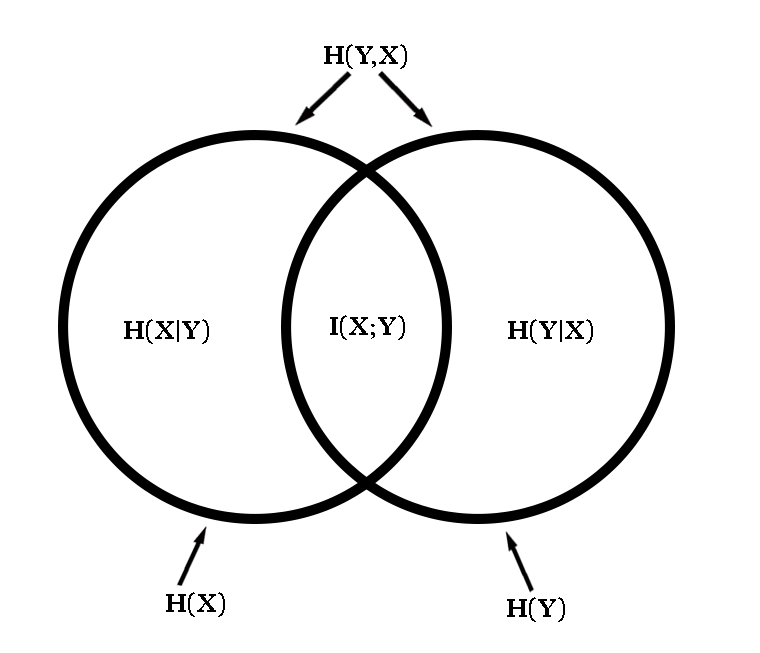
\includegraphics[width=8cm]{VennDiagram}
	\centering
	\caption{Venn Diagram}
\end{figure}

\section{Two looks}
\textbf{Here is a statement about pairwise independence and joint independence.  Let $X,Y_1$ and $Y_2$ be binary random variables.  If $I(X;Y_1)=0$ and $I(X;Y_2)=0$, does is follow that $I(X;Y_1,Y_2)=0$?}
\subsection{Yes or no?}
No
\subsection{Prove or provide a counterexample.}
If $X=Y_1$ XOR $Y_2$ then X is independent of $Y_1$, and independent of $Y_2$ but not independent of $(Y_1,Y_2)$ since if you have both $Y_1$ and $Y_2$ you could determine the true value of $X$.
\subsection{If $I(X; Y_1)=0$ and $I(X; Y_2)=0$ in the above problem, does it follow that $I(Y_1;Y_2)=0$?  In other words, if $Y_1$ is independent of $X$, and if $Y_2$ is independent of $X$, is it true that $Y_1$ and $Y_2$ are independent}
No.  Knowing that they are independent of X doesn't tell you anything about their relationship to each other.  If $Y_1 = Y_2$ then they could be both be individually independent of $X$ and completely dependent on each other.

\section{A measure of correlation}
\textbf{Let $X_1$ and $X_2$ be identically distributed, but not necessarily independent.  Let: $$\rho = 1-H(X_2|X_1)/H(X_1)$$}
\subsection{Show $\rho = I(X_1;X_2)/H(X_1)$}
Since $X_1$ and $X_2$ are identically distributed, we know that $H(X_1)=H(X_2)$
$$\rho = 1-H(X_2|X_1)/H(X_1) = (H(X_1)-H(X_2|X_1))/H(X_1)$$
$$\rho = (H(X_2)-H(X_2|X_1))/H(X_1)=I(X_1;X_2)/H(X_1)$$
\subsection{Show $0 \leq \rho \leq 1$}
$$0 \leq H(X_2|X_1) \leq H(X_2) = H(X_1)$$
$$0 \leq (H(X_1)-H(X_2|X1))/H(X_1) \leq 1$$
$$0 \leq \rho \leq 1$$
\subsection{When is $\rho=0$?}
$\rho=0$ iff $X_1$ and $X_2$ are independent.  That is, if $I(X_1;X_2)=0$
\subsection{When is $\rho=1$?}
$\rho =1$ iff $H(X_2|X_1)=0$.  That is if $X_2$ is a function of $X_1$.

\end{document}  